\begin{figure*}[th!]
    \centering
    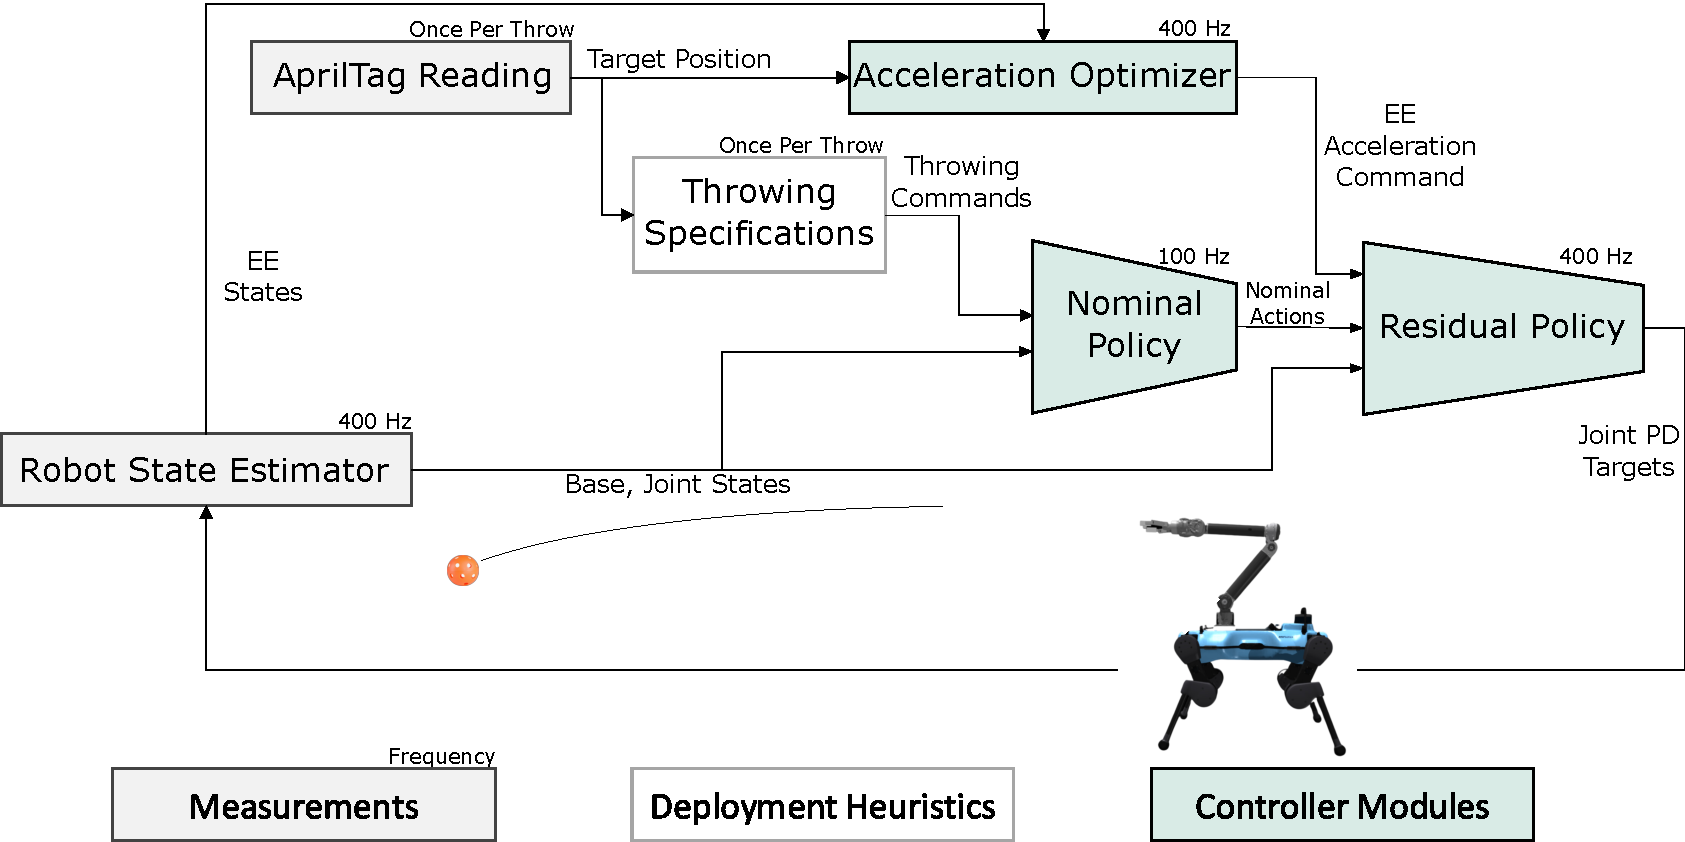
\includegraphics[width=0.75\textwidth]{figures/pipeline/pipeline1.pdf}
    \caption{\textbf{The proposed control framework.} consists of a standard whole-body base throwing policy, a residual policy, and an acceleration optimizer. The latter two modules run at the same frequency as the robot state estimation to provide high-frequency state feedback for the throwing motion. During the deployment, the controller acquires the target position from the AprilTag reader and computes the PD target commands for each joint on the robot.}
    \label{fig:pipeline}

    % \vspace{1.5cm}
\end{figure*}